  In the previous sections we have been working with a single domain denoted by $X$. Intuitively, it might be useful to think about the domain as the different values of a property (independently of the object that has that property). For example, we could say that for the property \textit{length} the domain is $\R^+\coleq
  \{x\in\R \mid x \geq 0\}$ and a person might have a \textit{height} defined in that domain (modeled as a fuzzy set), although not all length values will be compatible with a person's height since it is safe to assume impossible to be 10 meters tall, but we do not know where to place a sharp boundary, so the feasible region of heights is best represented by a fuzzy set. If we were to look at the arm length, then we would have another set of feasible lengths. Treating each set independently, does not allow distinguishing between the people of the same height with different arm length or vice versa. Therefore, it is needed to a way to differentiate each unique combination of attributes. Notice that in this example, height and arm length have the same domain but for example hair color would have a different domain.\\

  Mathematically, this is done with relations which are subsets of the Cartesian product of the domains, so that each element is a unique possible combination of attributes, an ordered n-tuple. For simplicity, let us consider just the Cartesian product of 2 sets since the general case can be obtained inductively (see remark below). Again, the ``fuzzy" part will be referred to how we generalize the membership values to the continuum.


  \begin{definition}[Fuzzy Relation]
    Let $X\neq \emptyset \neq Y$ be classical sets. Then a fuzzy relation $R$ is a fuzzy set on $X\times Y$, i.e., $R\in \fuzzy{X\times Y}$. $R(x,y)$ will denote the degree of membership of $(x,y) \in R$.
  \end{definition}

  \begin{notation}[label={not:compositionFS}]{Notation}
    Although Fuzzy Relations are Fuzzy Sets as well, the name distinction will be used to denote whether the domain is a Cartesian product or not.
  \end{notation}

  \begin{remark}
    To formally extend the Cartesian product from two sets to \( n \) sets using induction, it is important to observe that it satisfies associativity up to a natural isomorphism, i.e., 
    \[
    (A\times B)\times C \cong A\times (B\times C).
    \]
    and that t-norms satisfy the associativity property.
  \end{remark}

  Before giving the definition of the fuzzy Cartesian product, we need to first understand what the classical Cartesian product is in terms of the membership function. When we define a Cartesian product $A\times B$ as "\textit{all unique ordered pairs of elements from $A$ \textbf{and} $B$}", in terms of membership functions we are taking the intersection of membership to $A$ and membership to $B$. Therefore, generalizing that notion with a t-norm we get the following definition.

  \begin{definition}[Fuzzy Cartesian Product]
    It is a fuzzy relation $A\times B \in \fuzzy{X\times Y}$ such that the membership function is given by:
    \[ 
    (A\times B)(x,y) = T(A(x), B(y)), \quad \forall (x,y) \in X\times Y
    \]
    where $T$ is a t-norm.
  \end{definition}

  To justify the definition of the membership function of a Cartesian product of two fuzzy sets, let us first recall that in classical sets, we can retrieve the orginal subsets individually by taking the projection of the Cartesian product. Given $R$ a relation on $X\times Y$ the projections are:

  \[\Pi_X(R)=\{x \in X \mid \exists y \in Y \textnormal{ such that } (x,y) \in R\}\]
  \[\Pi_Y(R)=\{y \in Y \mid \exists x \in X \textnormal{ such that } (x,y) \in R\}\]

  Then, with the boolean membership, it can be expressed as well as:

  \[\Pi_X(R)(x)=\sup\{R(x,y) \mid y\in Y\}=
  \begin{cases}
    1 & \textnormal{if } \exists y \in Y \textnormal{ such that } (x,y) \in R \\
    0 & \textnormal{otherwise}
  \end{cases}
  \]
  \[
    \Pi_Y(R)(y)=\sup\{R(x,y) \mid x\in X\}=
    \begin{cases}
      1 & \textnormal{if } \exists x \in X \textnormal{ such that } (x,y) \in R \\
      0 & \textnormal{otherwise}
    \end{cases}
  \]

  It is clear that in the case of having 2 possible values for the membership function, the above expresions are identical. The use of $\sup$ in the definition of the projection can be intuitively interpreted as the \textit{shadow} of the membership function of the Cartesian product, as figure \ref{fig:class_cart_prod} illustrates. It is also desirable because then the following property holds for any classical Cartesian product:\\
  $$ 
  \Pi_X(A\times B)=A \quad \textnormal{ and } \quad \Pi_Y(A\times B)=B \forall A\in X, \forall B \in Y
  $$

  \begin{figure}[ht]
    \centering
    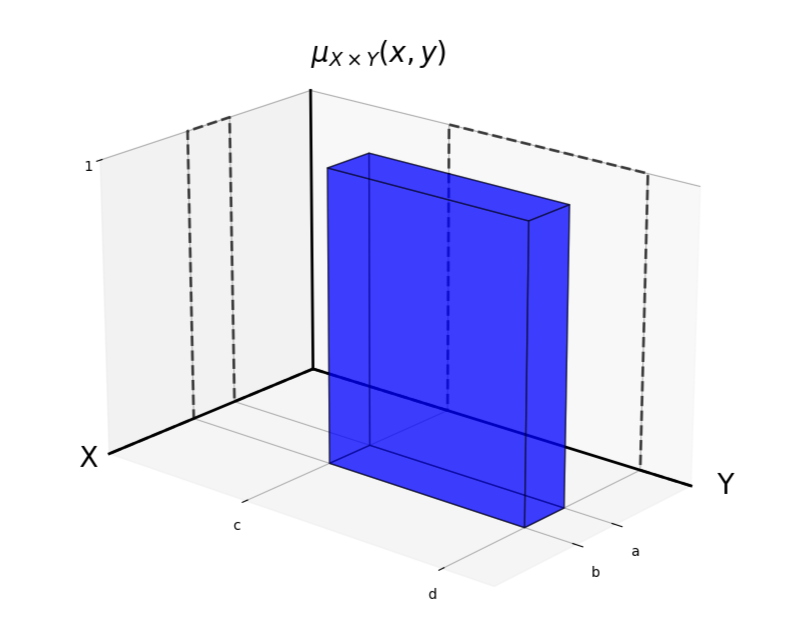
\includegraphics[width=0.65\textwidth]{ch1/figures/class_cart_prod.png}
    \caption{The blue volume represents the membership function of the Cartesian product of two classical sets $X=[a,b]$ and $Y=[c,d]$ in $\R$. In the plane $y=0$ we have the projection that corresponds to the membership function of $X$ and analogously, the projection of $Y$ in the plane $x=0$.}
    \label{fig:class_cart_prod}
  \end{figure}

  Therefore, we define:

  \begin{definition}[Projection of a fuzzy relation]
    The projection from fuzzy relations on $X\times Y$ onto the fuzzy sets on $X$ is the function:
    \[
      \begin{aligned}
        \Pi_X: \fuzzy{X\times Y} &\longrightarrow \fuzzy{X} \\
        R &\longmapsto \Pi_X(R)
      \end{aligned}
    \]
    where $\Pi_X(R)(x) = \sup_{y\in Y}\{R(x,y)\}\forall x \in X$
  \end{definition}

  Applying the definition of projection with the supremum to fuzzy sets, we have a way to retrieve the membership function of each fuzzy set given the membership function of a fuzzy Cartesian product (figure \ref{fig:fuzzy_cart_prod}). Therefore, any fuzzy Cartesian product can be expressed as the fuzzy Cartesian product of its own projections. This is justified in the following proposition: \\






  \begin{figure}[ht]
      \centering
      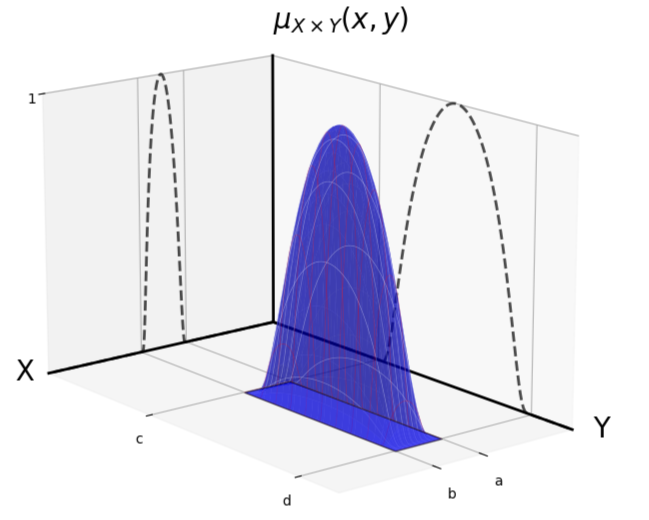
\includegraphics[width=0.65\textwidth]{ch1/figures/fuzzy_cart_prod.png}
      \caption{The blue volume represents the membership function of the Cartesian product of two fuzzy sets $X$ and $Y$. In the plane $y=0$, we have the projection that corresponds to the membership function of $X$, and analogously, the projection of $Y$ in the plane $x=0$. The partial memberships illustrate how the fuzzy relations can vary across the domains.}
      \label{fig:fuzzy_cart_prod}
  \end{figure}



\begin{proposition}[Retrieval of Fuzzy Sets from their T-norm Cartesian Product]
  Let $A \in \fuzzy{X}$ and $B \in \fuzzy{Y}$ be fuzzy sets and $T$ a left-continuous t-norm. If the fuzzy set $B$ is normalized (i.e., $\sup\{B(y) \mid y \in Y\}  = 1$), then $\Pi_X(A \times B)(x) = A(x)$ for all $x \in X$. 
  In general, if $B$ is not normalized, we only get a lower bound $\Pi_X(A \times B)(x) \le A(x)$.
  \end{proposition}
  
  \begin{proof}
  \begin{equation*}
    \begin{split}
      \Pi_X(A \times B)(x) &= \sup_{y \in Y} T(A(x), B(y))= \\
      &= T(A(x), \sup_{y \in Y} B(y)) \leq
      \begin{cases}
        \min(A(x), 1) = A(x) & \text{if } B \text{ is normalized}\\
        \min(A(x), \sup_{y \in Y} B(y)) \leq A(x) & \text{otherwise}
      \end{cases}
    \end{split}
  \end{equation*}
  Since $A(x)$ is a constant with respect to the supremum over $y$, and t-norms are non-decreasing and left-continuous\footnote{If the function were only left-continuous but not non-decreasing, then that equality would instead be the $\geq$ inequality.} in their second argument, then the second equality holds. The inequality before the cases is justified using that the minimum t-norm is the strongest t-norm.
  \end{proof}
  
  \begin{remark}
  It is also crucial to emphasize that this retrieval is meaningful when the fuzzy relation $R$ under consideration is indeed a fuzzy Cartesian product of the form $A \times B$ using the t-norm $T$. If a given fuzzy relation $R'$ on $X \times Y$ is not $T$-decomposable (i.e., it cannot be expressed as $T(A'(x), B'(y))$ for any fuzzy sets $A'$ on $X$ and $B'$ on $Y$ with respect to the t-norm $T$), then the notion of retrieving original sets $A'$ and $B'$ from $R'$ does not make sense. While one can always compute the projections $A_P(x) = \Pi_X(R')(x)$ and $B_P(y) = \Pi_Y(R')(y)$, the relation $R'$ will not necessarily be equal to the $T$-Cartesian product of its projections, i.e., $R'(x,y) \neq T(A_P(x), B_P(y))$ in general for non-decomposable relations.
  \end{remark}


  Since infinitely many relations (including those that are not a fuzzy Cartesian product) may have the same projections, it is not possible define the inverse operation. However, in the literature \cite[p.~61]{HistoryFL2017}, it is also defined the cylindric extension of a fuzzy set $A\in\fuzzy{X}$ as $CE_X(A)(x,y) = A(x)$. This operation is the simplest way to extend a fuzzy set to a relation ($\Pi_X(CE_X(A))=A$), and can be generalized to any n-ary relation as well.\\



\subsubsection*{Types of Fuzzy Relations on a Single Set}

When a binary fuzzy relation $R$ is defined on the Cartesian product of a single set with itself, it can characterize various ways in which elements of $X$ relate to themselves. Several properties, analogous to those in classical relations, are important for classifying these fuzzy relations \cite[p.~66]{HistoryFL2017}.

\begin{definition}[Properties of Binary Fuzzy Relations on $X^2$] Let $R \in \fuzzy{X \times X}$ (or $R \in \fuzzy{X^2}$) be a fuzzy binary relation, then:
  \begin{itemize}
    \item $R$ is \textbf{reflexive} if $R(x,x) = 1$ for all $x \in X$.
          Intuitively, every element is fully related to itself.
    \item $R$ is \textbf{symmetric} if $R(x,y) = R(y,x)$ for all $x,y \in X$.
          Intuitively, the degree of relationship from $x$ to $y$ is the same as from $y$ to $x$.
    \item $R$ is \textbf{transitive} (specifically, transitive under a t-norm $T$) if for all $x,y,z \in X$ and a given t-norm $T$,
          \[ T(R(x,y), R(y,z)) \le R(x,z). \]
          Using the definition of composition (see definition \ref{def:compos}) this can be expressed as $R \supseteq R \circ R$. Often the minimum t-norm is used and it is then called sup-min transitive.
  \end{itemize}
\end{definition}

Based on these properties, two important types of fuzzy relations are:

\begin{definition}[Fuzzy equivalence relation]
  A fuzzy relation $S \in \fuzzy{X \times X}$ is a fuzzy equivalence relation (also called similarity relation) if it is reflexive, symmetric, and transitive (typically sup-min transitive).
\end{definition}
It generalizes the concept of a classical equivalence relation to the fuzzy context, indicating the degree to which elements are considered ``similar" or ``equivalent."

\begin{definition}[Fuzzy Compatibility Relation]
  A fuzzy relation $C \in \fuzzy{X \times X}$ is a \textbf{fuzzy compatibility relation} (also sometimes called a tolerance or proximity relation) if it is reflexive and symmetric.
\end{definition}
A fuzzy compatibility relation indicates that elements are compatible or close to each other, but this compatibility is not transitive. If $x$ is compatible with $y$, and $y$ with $z$, $x$ is not necessarily compatible with $z$ to the same degree.










\subsection{Composition of Fuzzy Sets}
\label{sec:compos}

The concept of projection allows us to combine fuzzy relations sharing a common domain. Intuitively, composing two fuzzy relations involves intersecting their membership values (using a t-norm) and then projecting the result onto the domain where the relations do not overlap.

\begin{definition}[Composition of Two Fuzzy Relations]\label{def:compos}
    Let \( R \in \fuzzy{X \times Y} \) and \( G \in \fuzzy{Y \times Z} \) be fuzzy relations sharing the set \(Y\). Their composition \( R \circ G \) is the fuzzy relation in \(\fuzzy{X \times Z}\) defined by
    \[
    (R \circ G)(x,z) = \Pi_{X\times Z}\Bigl[\, T\bigl(R(x,y), G(y,z)\bigr) \Bigr] = \sup_{y\in Y}\, T\bigl(R(x,y), G(y,z)\bigr),
    \]
    where \(T\) is a t-norm acting as the fuzzy intersection.
\end{definition}

% This means that given three properties $X$, $Y$ and $Z$ and two fuzzy relation R from X to Y and another fuzzy relation from Y to Z, we have a way to induce a relation $R\circ G$ between X and Z.

% (add a diagram here)

Given three sets \(X\), \(Y\), and \(Z\), suppose we have a fuzzy relation \(R\) from \(X\) to \(Y\) and another fuzzy relation \(G\) from \(Y\) to \(Z\). Using the composition operation, we can derive a new fuzzy relation \(R \circ G\) that directly connects \(X\) to \(Z\).

\noindent
\begin{minipage}{0.7\textwidth}
In this diagram, the arrows represent fuzzy relations, with \(R\) mapping elements from \(X\) to \(Y\), \(G\) mapping from \(Y\) to \(Z\), and \(R \circ G\) representing the induced fuzzy relation between \(X\) and \(Z\) through composition.\\
\end{minipage}%
\begin{minipage}{0.3\textwidth}
  \begin{center}
    \begin{tikzcd}
      X \arrow[r, "R", leftrightarrow] & Y \arrow[r, "G", leftrightarrow] & Z \arrow[bend right=30, from=1-1, "R \circ G"', leftrightarrow]
      \end{tikzcd}
  \end{center}

\end{minipage}


We can define the composition of a fuzzy set with a fuzzy relation in a completely analogous way. 

\begin{definition}[Composition of a Fuzzy Set and a Fuzzy Relation]
    Let \( A \in \fuzzy{X} \) be a fuzzy set on \(X\) and \( R \in \fuzzy{X \times Y} \) be a fuzzy relation between \(X\) and \(Y\). The composition \( A \circ R \in \fuzzy{Y} \) is defined by
    \[
    (A \circ R)(y) = \Pi_{Y}\Bigl[\, T\bigl( A(x), R(x,y) \bigr) \Bigr] = \sup_{x \in X}\, T\bigl( A(x), R(x,y) \bigr),
    \]
    where \(T\) is a t-norm.
\end{definition}

\subsection{Extension Principle}
\label{sec:ext_pple}

Following a similar idea as in the definition of the composition of fuzzy sets, we can derive a way to generalize crisp functions to fuzzy sets.\\

Let us consider the crisp function $f:\,X \longrightarrow Y$ where $X$ and $Y$ are classical sets. We also consider the fuzzy sets $A \in \fuzzy{X}$. Then $f$ induces the classical relation $R=\{(x,y)\in X\times Y \mid f(x)=y\}$. And we can also make this relation fuzzy by copying the membership function of $A$:
$$ \mu_R (x,y) = \mu_A (x) \forall (x,y)\in R$$
Now we can define $B\in\fuzzy{Y}$, the fuzzy image of $A$ under $f$, as the projection of this fuzzy relation:
$$\mu_B (y) = \Pi_Y (R) = \sup\{R(x,y)\mid x\in X\} = \sup\{\mu_A (x)\mid x\in X, \, f(x)= y\} = \sup_{x\in f^{-1}(y)}\{\mu_A(x)\}$$

This is called the (Zadeh's) extension principle and is the basis for building arithmetic for fuzzy numbers (see section \ref{sec:fuzzy_numbers}) and generalizing any crisp function to fuzzy sets: 

\begin{definition}[Zadeh's extension principle]
  Let $f: X \longrightarrow Y$ be a crisp function and $A\in \fuzzy{X}$ a fuzzy set on $X$. Then we can define $f(A)\in \fuzzy{Y}$ as:
  \[
  \mu_{f(A)}(y)\equiv f(A)(y) = 
  \begin{cases}
    \sup_{x\in f^{-1}(y)}A(x) & \textnormal{if } f^{-1}(y)\neq \emptyset\\
    0 & \textnormal{otherwise}
  \end{cases}
  \quad\quad\quad \textnormal{where } f^{-1}(y)=\{x\in X \mid f(x)=y\}
  \]
\end{definition}


\begin{remark}
  If $f$ is \textbf{injective} then for any $y \in \textnormal{Im}(f)$ there exists a unique $x \in X$ such that $f(x)=y$, and therefore $f^{-1}(y)=\{x\}$. Then the first case can be rewritten as, $f(A)(y) = A(f^{-1}(y))$ if $y \in \textnormal{Im}(f)$.
\end{remark}

It is important to highlight as well that this definition is a straightforward generalization of set-valued functions where $f(A)= \{f(x)\mid x\in A\}$. In terms of boolean membership function:
$$\chi _{f(A)}(y)=\sup_{x\in f^{-1}(y)}\chi_A(x)$$

The definition above can be generalized to vector functions using the definition of fuzzy Cartesian product, which requires us to take the intersection (using a t-norm):

\begin{definition}[Sup-T extension principle]
  Let $f: X_1 \times \cdots \times X_n \longrightarrow Y$ be a crisp function and $A_1 \in \fuzzy{X_1}, \ldots, A_n \in \fuzzy{X_n}$ be fuzzy sets. Then we can define $f(A_1,\ldots,A_n)\in \fuzzy{Y}$ as:
  \[
  \mu_{f(A_1,\ldots,A_n)}(y)\equiv f(A_1,\ldots,A_n)(y) = 
  \begin{cases}
    \sup_{(x_1,\ldots,x_n)\in f^{-1}(y)} T(A_1(x_1),\ldots,A_n(x_n)) & \textnormal{if } f^{-1}(y)\neq \emptyset\\
    0 & \textnormal{otherwise}
  \end{cases}
  \]
  where $f^{-1}(y)=\{(x_1,\ldots,x_n)\in X_1\times\cdots\times X_n \mid f(x_1,\ldots,x_n)=y\}$ and $T$ is a t-norm.
\end{definition}

Which is again a generalization of vector set-valued functions where: $$f(A_1,\ldots,A_n)= \{f(x_1,\ldots,x_n)\mid x_i\in A_i\}$$
In terms of boolean membership function:
$$\chi _{f(A_1,\ldots,A_n)}(y)=\sup_{(x_1,\ldots,x_n)\in f^{-1}(y)}T(\chi_{A_1}(x_1),\ldots,\chi_{A_n}(x_n)) = \sup_{(x_1,\ldots,x_n)\in f^{-1}(y)}min\{\chi_{A_1}(x_1),\ldots,\chi_{A_n}(x_n)\}$$

Where we have used that every t-norm operates the same on boolean memberships.\\

Alternative extension principles have been proposed in the literature for two main reasons: seeking higher computational efficiency and avoiding uncertainty ``inflation''. The latter is due to the principle treating each of the variables independently, which leads to criticized edge cases such as the one shown in example \ref{ex:unc_inflation}. Nevertheless, none of them are explored in this work.